\begin{figure}[htbp]
\centering 
%   \subfloat[Parameter space plot, \acs{SCT}, $\sigma_n=1068$ Pa, P=1.0.]{
% 	  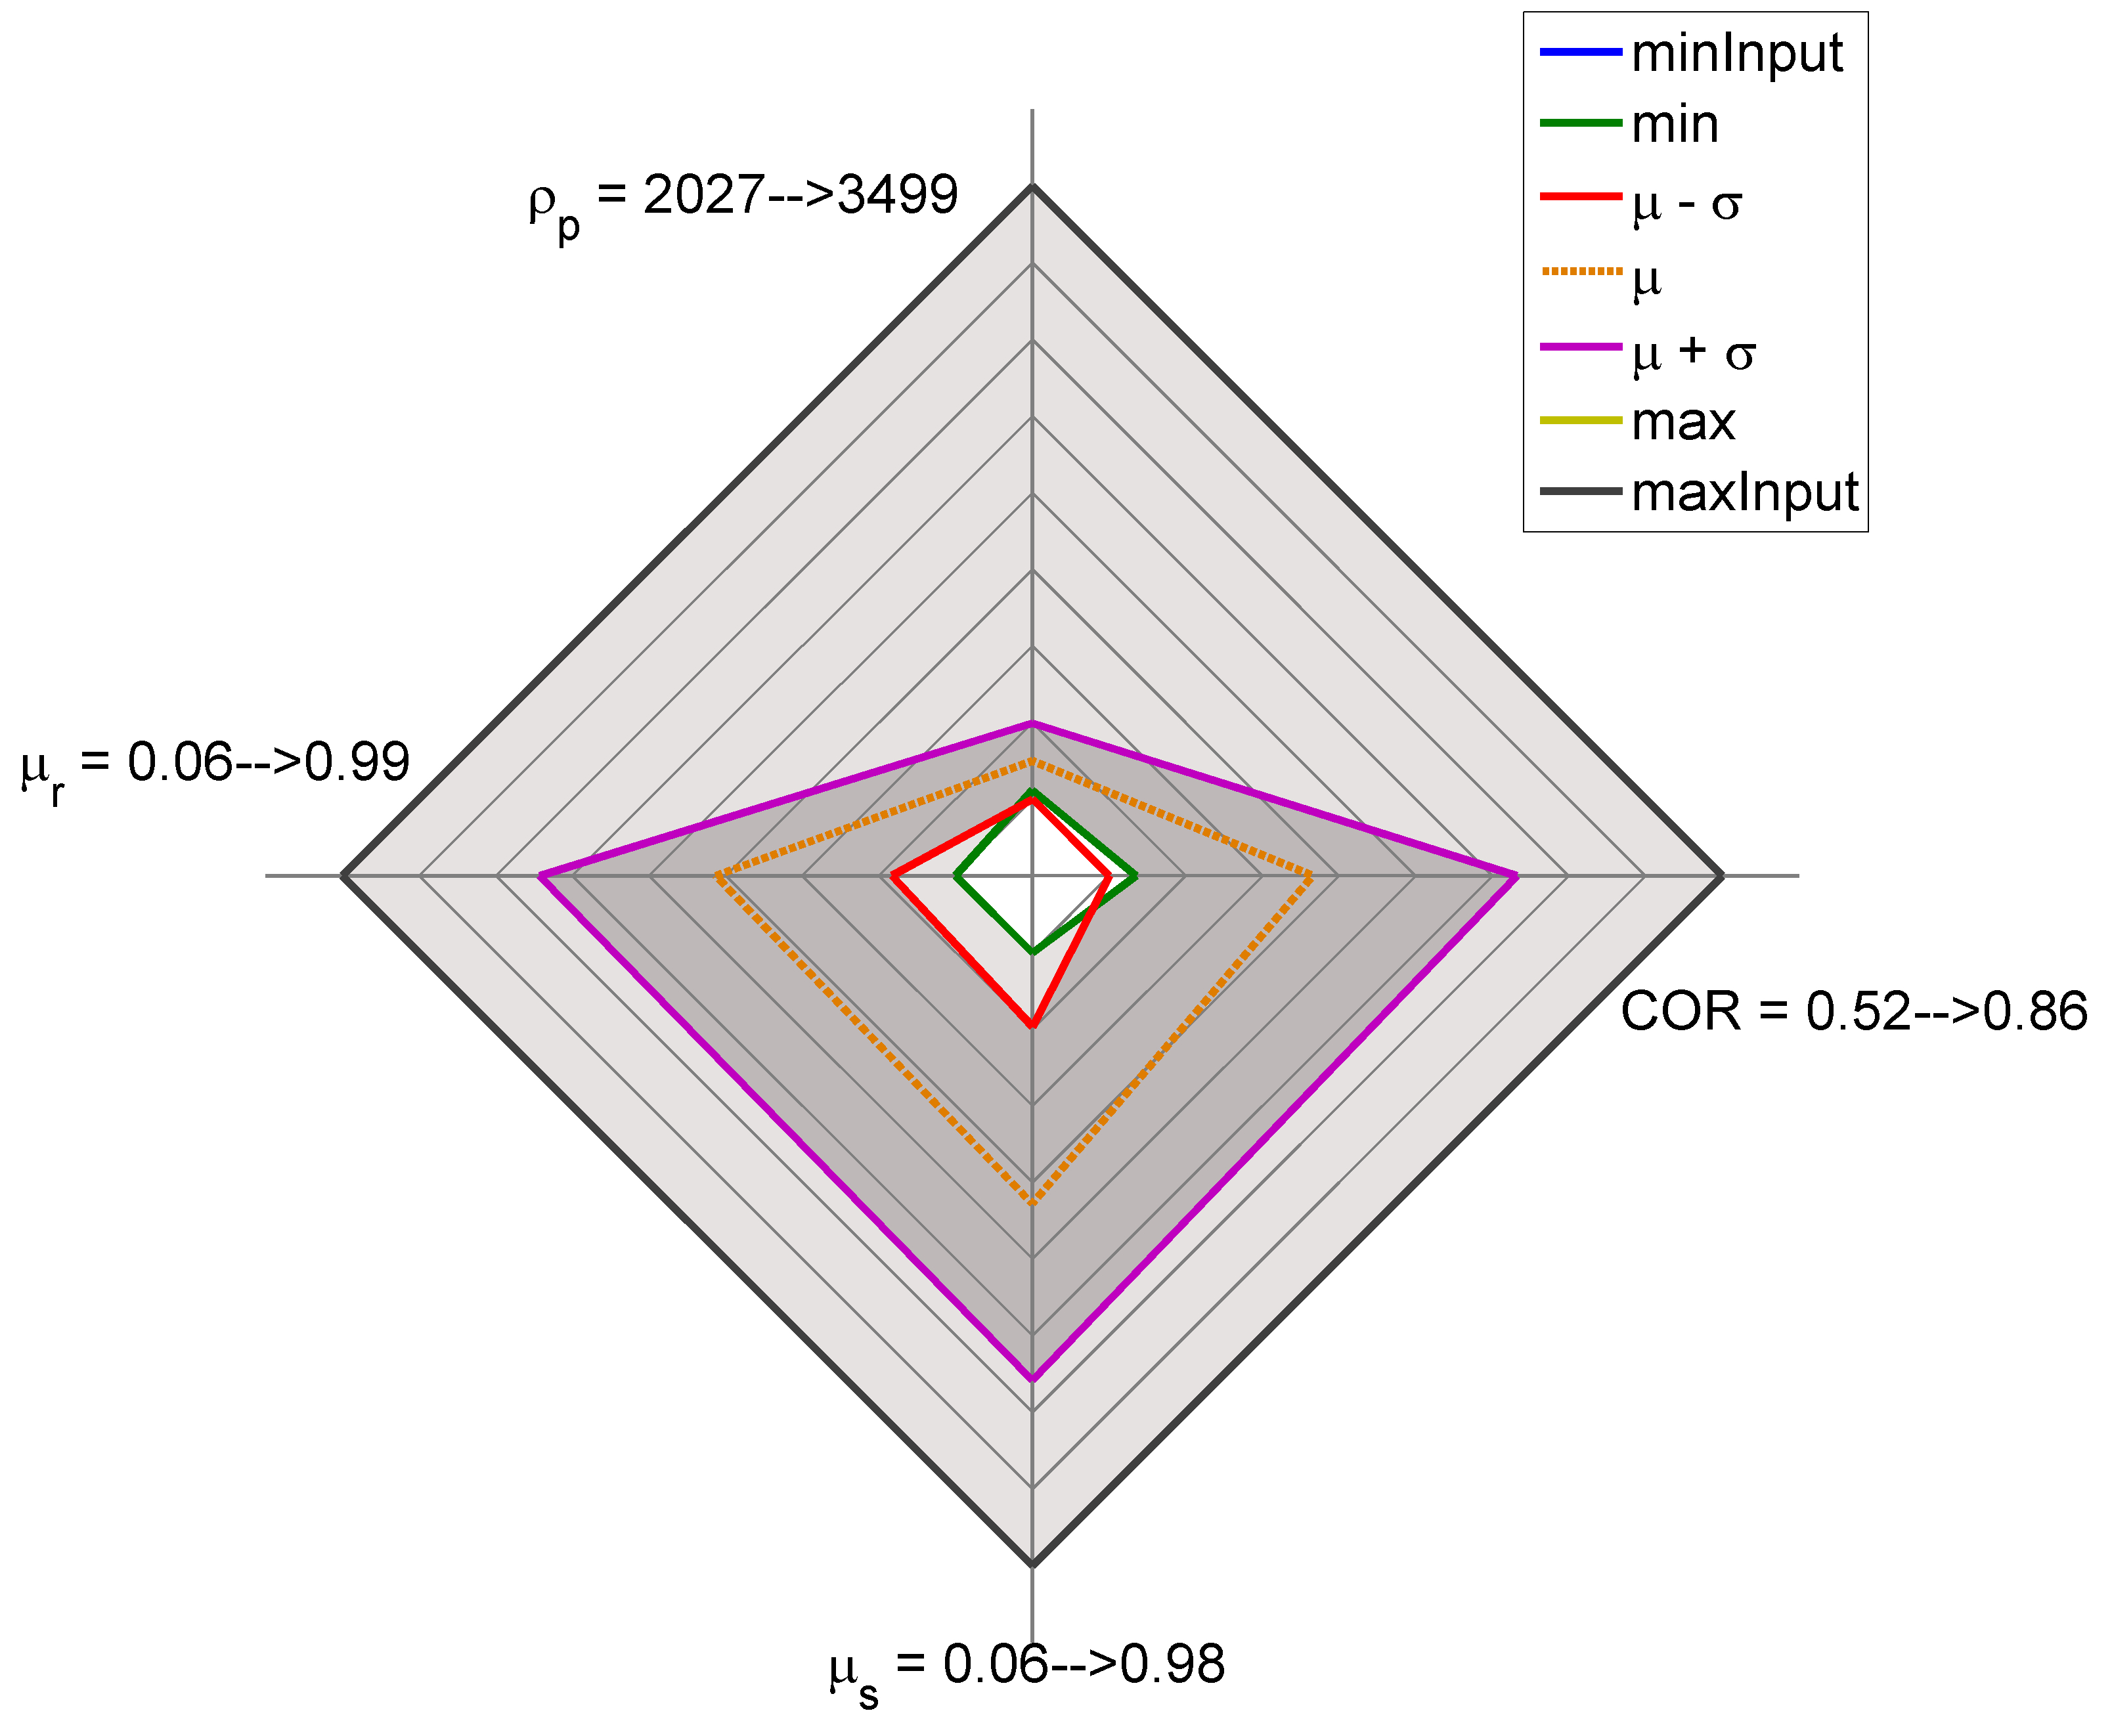
\includegraphics[width=.35\columnwidth]{images/041radarpirker1schulze1068}
% 	  \label{fig:041radarpirker1schulze1068}
%   }
%   \\157BoxSCT10070p08sinterfine.png
%158BoxSCT10070p12sinterfine.png
    \subfloat[Box plot, \acs{SCT}, $\sigma_n=10070$ Pa, P=0.8.]{
	  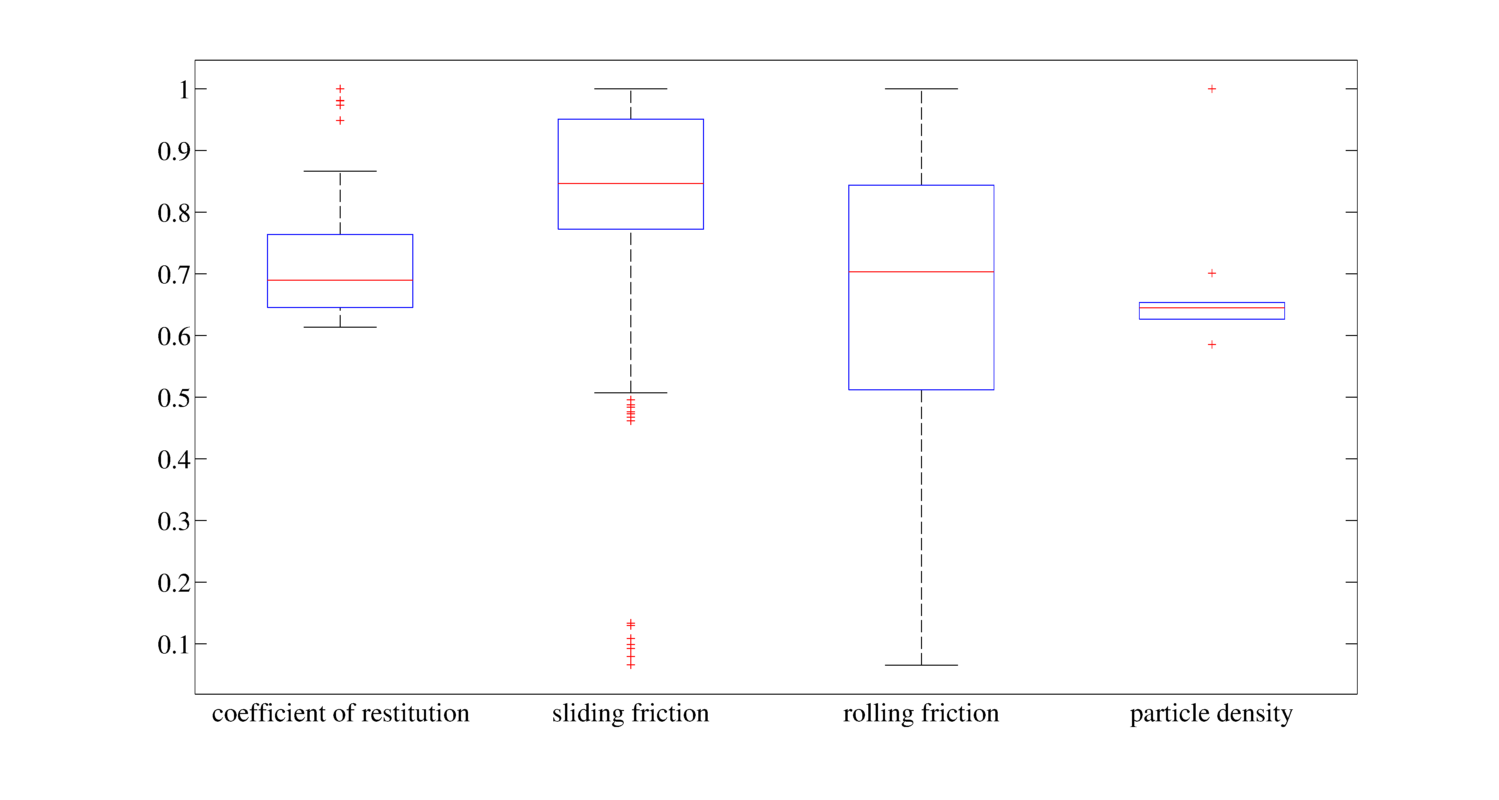
\includegraphics[width=.70\columnwidth]{images/157BoxSCT10070p08sinterfine}
	  \label{fig:157BoxSCT10070p08sinterfine}  }
  \\
    \subfloat[Box plot, \acs{SCT}, $\sigma_n=10070$ Pa, P=1.0.]{
	  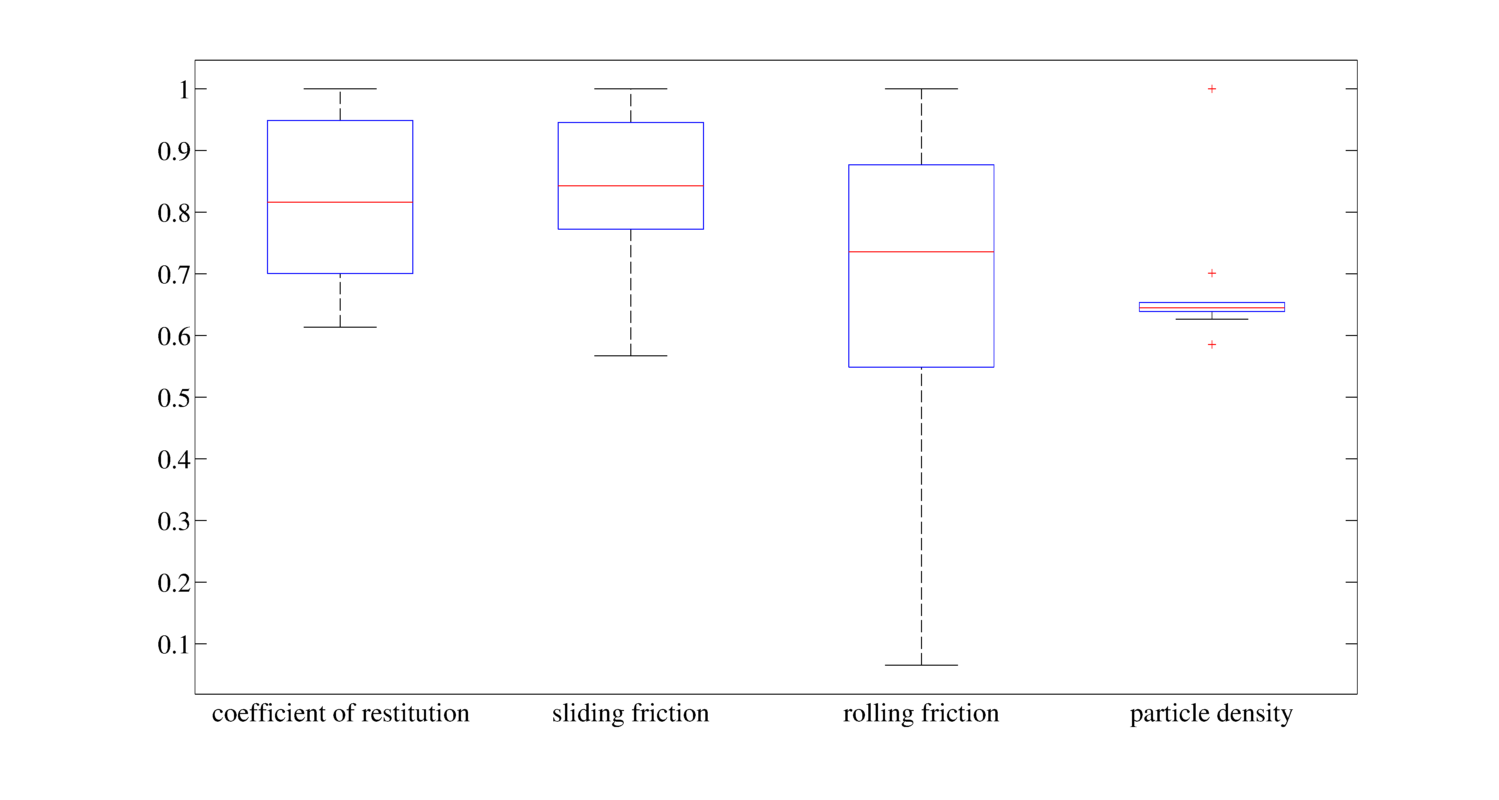
\includegraphics[width=.70\columnwidth]{images/075sctboxplot}
	  \label{fig:075sctboxplot}  }
  \\
    \subfloat[Box plot, \acs{SCT}, $\sigma_n=10070$ Pa, P=1.2.]{
	  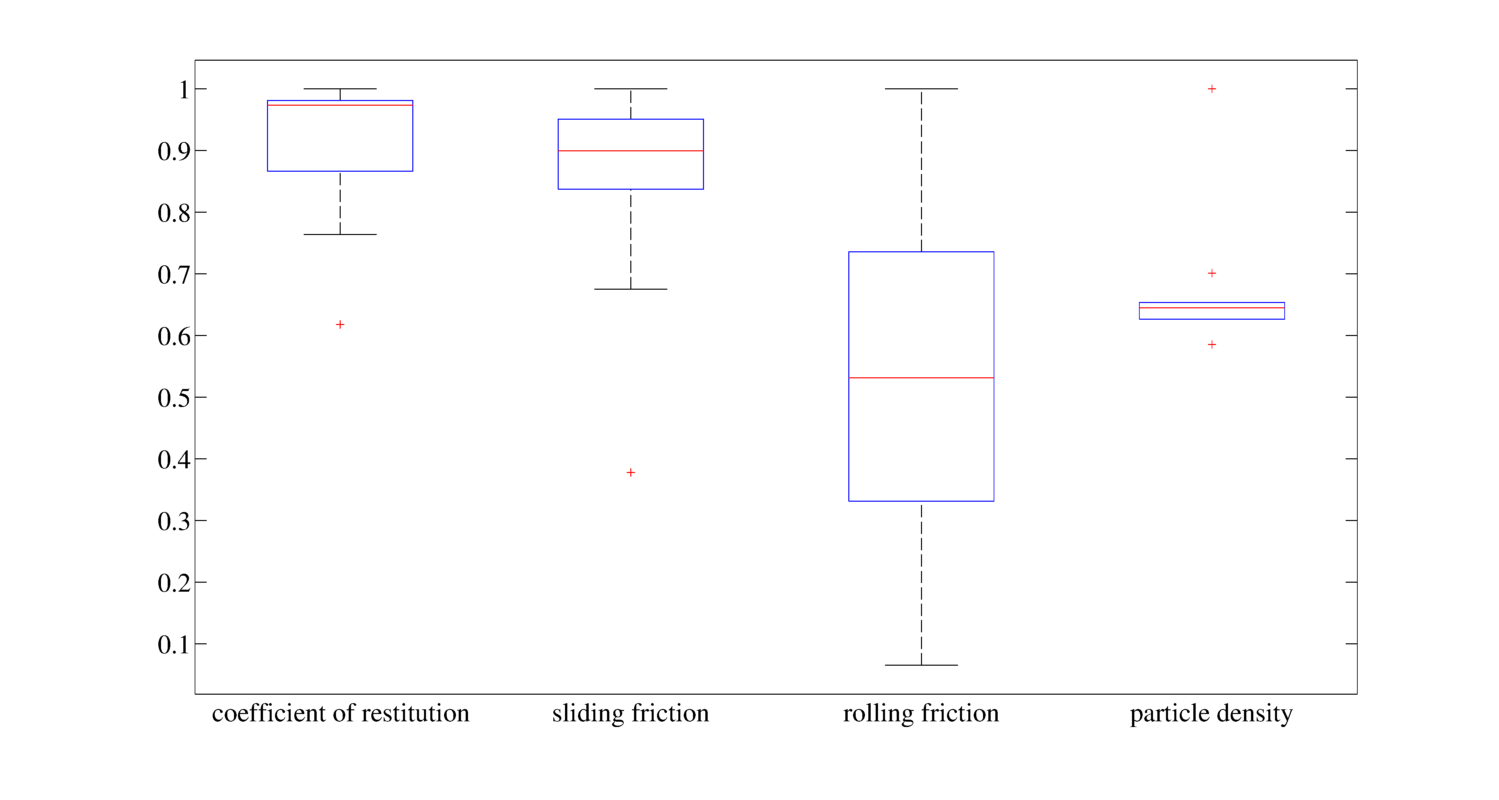
\includegraphics[width=.70\columnwidth]{images/158BoxSCT10070p12sinterfine}
	  \label{fig:158BoxSCT10070p12sinterfine}  }
  \\
  \caption[SCT box plots for sinter fine]{SCT box
  plots for sinter fine, $\sigma_n=10070$ Pa. The range of valid parameters is
  shown, together with the average and the 25 and 75 percentile.}
  \label{fig:156boxplotsct10070sinterfine}
\end{figure}